%!TEX root = ../paper.tex
\chapter{DVB-T发射端}
	\section{能量扩散}
		\par 当发射的信号过于集中在某一频段上,将对与其共用频段的其他系统或设备造成较大干扰。人为地对发射信号进行随机化或者加扰,可以使原本集中的信号能量均匀分布。同时,由于添加的随机码为伪随机码,具有确定性的算法,所以在接收端很容易进行去随机化,解出正确的信息。在数字通信过程中,通过添加伪随机信号还能缩短连续的“0”或者连续的“1”的长度,接收端提取定时信号将变得更加容易\cite{数字电视DVB标准能量扩散的FPGA设计与实现_肖闽进}。
		\par MPEG-2的传输复用包长为188字节,包括一个同步字节,如图\ref{fig:MPEG_2_TS}所示。		
		\begin{figure}[thb]
	\centering
	\begin{tikzpicture}
		\node(SYNC)[rectangle,draw=black,text centered,minimum height=1cm,minimum width=2cm,label=below:1字节]{SYNC};
		\node(data)[rectangle,draw=black,text centered,right = 0 of SYNC,minimum height=1cm,minimum width=8cm,label=below:187字节]{MPEG-2传输数据};
	\end{tikzpicture}
	\caption{MPEG-2传输包}
	\label{fig:MPEG_2_TS}
\end{figure}
\endinput
		\par 其中同步字节为0x47,传送时从高位开始送入,即从0x47(0100 0111)的0开始送入,由伪随机二进制序列(PRBS,Pseudo Random Binary Sequence)和码流数据按位异或完成,结构如图\ref{fig:PRBS}所示。
		\begin{figure}[thb]
	\centering
	\begin{tikzpicture}[circuit logic US]
		\node (data)[rectangle split,rectangle split horizontal,rectangle split parts=15,draw,text width=0.4cm] at (0,0){
			\nodepart{text}1\nodepart{two}2\nodepart{three}3\nodepart{four}4\nodepart{five}5\nodepart{six}6\nodepart{seven}7\nodepart{eight}8\nodepart{nine}9\nodepart{ten}10\nodepart{eleven}11\nodepart{twelve}12\nodepart{thirteen}13\nodepart{fourteen}14\nodepart{fifteen}15
		};
		\node (comment1)[above=0.1cm of data,rectangle split,rectangle split horizontal,rectangle split parts=15,text width=0.4cm]{
			\nodepart{text}1\nodepart{two}0\nodepart{three}0\nodepart{four}1\nodepart{five}0\nodepart{six}1\nodepart{seven}0\nodepart{eight}1\nodepart{nine}0\nodepart{ten}0\nodepart{eleven}0\nodepart{twelve}0\nodepart{thirteen}0\nodepart{fourteen}0\nodepart{fifteen}0
		};
		\node (xor1)[xor gate,point left] at (3,-1){};
		\node (xor2)[xor gate,point right] at (2,-2.1){};
		\node (and)[and gate,point right] at (0,-2){};
		\node (enable) at (-1,-3) {使能};
		\node (input) at (1,-3.5) {输入数据};
		\node (output) at (5,-2.1) {随机化后的数据};
		\node (comment2) at (1,-1.3) {0 0 0 0 0 0 1 1......};
		
		\draw (data.fourteen south) |- (xor1.input 2);
		\draw (data.east) -| ++(1,-1) |- (xor1.input 1);
		\draw (data.text west) -| (-0.8*8,-1) |- (xor1.output);
		\draw (-0.8*8,-1) |- (and.input 1);
		\draw (enable.north) |- (and.input 2);
		\draw (and.output) -- (xor2.input 1);
		\draw (input.north) |- (xor2.input 2);
		\draw (xor2.output) -- (output.west);
		\fill (-0.8*8,-1) circle (2pt);
	\end{tikzpicture}
	\caption{能量扩散原理图}
	\label{fig:PRBS}
\end{figure}
\endinput
		\par 伪随机二进制序列的生成多项式为$g(x)=1+X^{14}+X^{15}$,伪随机寄存器中的初始序列是“1001 0101 0000 000”(在编程时可以定义为0xa9左移送入,而不用定义为0x4a80右移送入,减少一定的性能开销)。伪随机寄存器每8个传输包($8*188=1504$字节)作为一组,每8个传输包初始化一次,同时,对每组的第一个包的同步字节按比特取反,即同步字节由0x47变为0xB8。能量扩散从每组第1个传输包的同步字节之后的第1个比特开始进行,但在随后的7个传输包中的同步字节,不对输入的同步字节进行加扰,同步字节保持原状,仅仅产生伪随机码,这样能量扩散的周期就为$188*8-1=1503$字节。当输入码流不是MPEG-2 TS码流格式或者码流中断时,能量扩散继续进行,插入同步字节与空白字节完成来空包处理,这样接收端辨别出全零的空包并将其删除,就完成了整个能量扩散的过程。
		\par 程序实现主要代码见代码\ref{code:prbs}:
		\begin{lstlisting}[caption = {能量扩散}, label = {code:prbs}, language = C++ ]
void dvbt_energy_dispersal_impl::clock_prbs(int clocks)
{
	int res = 0;
	int feedback = 0;

	for (int i = 0; i < clocks; i++) {
	feedback = ((d_reg >> (14 - 1)) ^ (d_reg >> (15 - 1))) & 0x1;
	d_reg = ((d_reg << 1) | feedback) & 0x7fff;
	res = (res << 1) | feedback;
	}
	return res;
}
		\end{lstlisting}
	\section{RS编码}
		\par DVB-T系统的外编码采用RS编码(Reed-Solomon codes),由$k$个信息符号按一定关系组成$n$个符号,以$n$个符号为一组处理,是一种前向错误更正的信道编码。DVB-T系统使用的是由RS(255,239,$t$=8)衍生出的删余RS(204,188,$t$=8)码,通过对每个随机化后的188字节的传输包编码,通过生成多项式生成一个有效数据为188字节,总长度为204字节的误码保护包。RS编码从同步字节(0x47)或者倒相后的同步字节(0xB8)开始,误码保护包的组成如图\ref{fig:rs_204_188},最多可以校正8个字节的随机误码错误\cite{RS编码器的设计与实现_游余新}。
		\begin{figure}[thb]
	\centering
	\begin{tikzpicture}
		\node (sync)[rectangle,draw] at (0,0) {$\overline{\text{SYNC}}or\text{SYNC}_n$(1字节)};
		\node (data)[rectangle,draw,right=0 of sync]{随机化数据(187字节)};
		\node (check)[rectangle,draw,right=0 of data]{奇偶检验位(16字节)};
		\node (comment1) at (5,-1){204字节};
		\node (arrow1)[below = 0.1cm of sync.south west]{};
		\node (arrow2)[below = 0.1cm of check.south east]{};

		\draw [|<->|](arrow1) -- (arrow2);
	\end{tikzpicture}
	\caption{RS(204,188,8)误码保护包}
	\label{fig:rs_204_188}
\end{figure}
\endinput
		\par RS码生成多项式为:
		\begin{equation}
			g(x)=(x+\lambda ^0)(x+\lambda ^1)(x+\lambda ^2)...(x+\lambda ^{15})
		\end{equation}
		\par 其中$\lambda$=0x02。
		\par 域生成多项式为:
		\begin{equation}
			p(x)=x^8+x^4+x^3+x^2+1
		\end{equation}
		\par 可以在传输包前面增加51个全零字节,通过RS(255,239,$t$=8)编码器,再删除无用的全零字节,最终可以产生长度为204字节的RS码字。
		\par RS编码初始化主要代码见代码\ref{code:rs_init},RS编码主要代码见代码\ref{code:rs_encode}。
		\begin{lstlisting}[caption = {RS编码初始化}, label={code:rs_init}, language = C++ ]
void dvbt_reed_solomon::rs_init(int lambda, int n, int k, int t)
{
	d_n = n; d_k = k; d_t = t;
	// 2t = n - k, dmin = 2t + 1 = n -k + 1

	d_l = new unsigned char[d_n + 1];
	if (d_l == NULL) {
	std::cout << "Cannot allocate memory for d_l" << std::endl;
	exit(1);
	}

	d_g = new unsigned char[2 * d_t + 1];
	if (d_g == NULL) {
	std::cout << "Cannot allocate memory for d_g" << std::endl;
	delete [] d_l;
	exit(1);
	}

	//Generate roots of lambda
	d_l[0] = 1;

	for (int i = 1; i <= d_n; i++) {
	d_l[i] = gf_mul(d_l[i - 1], lambda);
	}

	//Init Generator polynomial buffer
	for (int i = 0; i <= (2*t); i++) {
	d_g[i] = 0;
	}

	//Start with x+lambda^0
	d_g[0] = 1;

	//Create generator polynomial
	for (int i = 1; i <= (2 * t); i++) {
	for (int j = i; j > 0; j--) {
		if (d_g[j] != 0) {
		d_g[j] = gf_add(d_g[j - 1], gf_mul(d_g[j], d_l[i - 1]));
		}
		else {
		d_g[j] = d_g[j - 1];
		}
	}

	d_g[0] = gf_mul(d_g[0], d_l[i - 1]);
	}

	// Init syndrome array
	d_syn = new unsigned char[2 * d_t + 1];
	if (d_syn == NULL) {
	std::cout << "Cannot allocate memory for d_syn" << std::endl;
	delete [] d_g;
	delete [] d_l;
	exit(1);
	}
}
		\end{lstlisting}
		\begin{lstlisting}[caption = {RS编码}, label = {code:rs_encode}, language = C++ ]
int dvbt_reed_solomon::rs_encode(unsigned char *data_in, unsigned char *parity)
{
	memset(parity, 0, 2 * d_t);

	for (int i = 0; i < d_k; i++) {
	int feedback = gf_add(data_in[i], parity[0]);

	if (feedback != 0) {
		for (int j = 1; j < (2 * d_t); j++) {
		if (d_g[2 * d_t - j] != 0) {
			parity[j] = gf_add(parity[j], gf_mul(feedback, d_g[2 * d_t - j]));
		}
		}
	}

	//Shift the register
	memmove(&parity[0], &parity[1], (2 * d_t) - 1);

	if (feedback != 0) {
		parity[2 * d_t - 1] = gf_mul(feedback, d_g[0]);
	}
	else {
		parity[2 * d_t - 1] = 0;
	}
	}

	return (0);
}
		\end{lstlisting}
	\section{卷积交织}
		\par DVB-T系统的外交织采用的是深度$I=12$,基数$M=17$的的卷积交织。以一个$M=3$的例子说明,此时卷积交织工作过程如图\ref{fig:convolutional_interleaver}所示。第一层直通,第二层有$M=3$个存储器,第三层有$2M=6$个存储器,输入、输出的每个字节由同步开关进行控制,第二层延时$M=3$个字节,第三层延时$2M=6$个字节,解交织的过程与此相反。输入输出数据流如图\ref{fig:convolutional_interleaver_data_structure}所示\cite{用FPGA实现DVB标准中的卷积交织_刘静},这样就将原来的数据分散发送了。
		\begin{figure}[thb]
	\centering
	\begin{tikzpicture}[align=center]
		\node (inputM3)[draw,text width=1.2cm] at (2,0) {M=3};
		\node (inputM6)[draw,text width=1.2cm] at (2,-1) {2M=6};

		\draw [arrow] (-1,0) -- (0,0) -- (1,1);
		\draw [arrow] (1,1) -- (3,1);
		\draw [arrow] (3,1) -- (4,0) -- (5,0);
		\draw [arrow] (0.75,0) -- (inputM3.west);
		\draw [arrow] (inputM3.east) -- (3.25,0);
		\draw [arrow] (0.75,-1) -- (inputM6.west);
		\draw [arrow] (inputM6.east) -- (3.25,-1);
	\end{tikzpicture}
	\caption{M=3时卷积交织图}
	\label{fig:convolutional_interleaver}
\end{figure}
\endinput
		\begin{figure}[thb]
	\centering
	\begin{tikzpicture}[align=center]
		\node (input1)[] at (0,2) {0,3,6};
		\node (input2)[] at (0,1) {1,4,7};
		\node (input3)[] at (0,0) {2,5,8};
		\node (output1)[] at (5,2) {0};
		\node (output2)[] at (5,1) {x};
		\node (output3)[] at (5,0) {x};
		\node (M3)[draw,text width=1.5cm] at (2.5,1) {M=3};
		\node (M6)[draw,text width=1.5cm] at (2.5,0) {2M=6};
		
		\node at (5.5,2) {3};
		\node at (6,2) {6};
		\foreach \x in {6.5,7,...,9.5}{
			\node at (\x,2) {\&};
		};
		\foreach \x in {5.5,6}{
			\node at (\x,1) {x};
		};
		
		\node at (6.5,1) {1};
		\node at (7,1) {4};
		\node at (7.5,1) {7};
		\foreach \x in {8,8.5,...,9.5}{
			\node at (\x,1) {\&};
		};
		
		\foreach \x in {5.5,6,...,7.5}{
			\node at (\x,0) {x};
		};
		\node at (8,0) {2};
		\node at (8.5,0) {5};
		\node at (9,0) {8};
		\node at (9.5,0) {\&};
		
		\draw [arrow](input1) -- (output1);
		\draw [arrow](input2) -- (M3.west);
		\draw [arrow](M3.east) -- (output2);
		\draw [arrow](input3) -- (M6.west);
		\draw [arrow](M6.east) -- (output3);
		
		\foreach \x in {5.25,5.75,...,9.25}{
			\draw [arrow](\x,2.5) -- (\x,-0.5);
		};
		
		\node at (0,-1) {输入数据流};
		\node at (6,-1) {输出数据流};

	\end{tikzpicture}
	\caption{卷积交织输入输出数据结构}
	\label{fig:convolutional_interleaver_data_structure}
\end{figure}
\endinput
		\par DVB-T系统中使用的卷积交织,$M=17$,即第一层直通,第二层延时$M=17$字节,第三层延时$2*17=34$字节...总共12层,其中同步字节$\text{SYNC}_n$)和倒相后的同步字节($\overline{\text{SYNC}}$总是经过第一层进行交织。
		\par 程序实现主要代码见代码\ref{code:convolutional_interleaver}。
		\begin{lstlisting}[caption = {卷积交织},label = {code:convolutional_interleaver},language = C++ ]
int dvbt_convolutional_interleaver_impl::work (int noutput_items,
				gr_vector_const_void_star &input_items,
				gr_vector_void_star &output_items)
{
	const unsigned char *in = (const unsigned char *) input_items[0];
	unsigned char *out = (unsigned char *) output_items[0];

	for (int i = 0; i < (noutput_items / d_I); i++) {
	//Process one block of I symbols
	for (unsigned int j = 0; j < d_shift.size(); j++) {
		d_shift[j]->push_front(in[(d_I * i) + j]);
		out[(d_I * i) + j] = d_shift[j]->back();
		d_shift[j]->pop_back();
	}
	}
	return noutput_items;
}
		\end{lstlisting}
	\section{内编码(卷积编码)}
		% TODO: fix
		\par DVB-T系统的内编码采用卷积编码,卷积码是由$k$个信息比特编码成$n(n>k)$比特码组,编码出的$n$比特的码组值,不仅与当前码字中的$k$个信息比特值有关,而且与其前面$N-1$个码字中的$(N-1)xk$个信息比特值有关,也即当前码组内的$n$个码元,它们的值取决于$N$个码组内的全部信息码元,$N$可称为卷积码编码的约束长度。
		\par DVB-T系统可以选择几种由码率为1/2的主卷积码删余后的卷积码。无论是等级或非等级传送模式,对于某一给定业务的数据率,系统可选择最适当的码率。主码的生成多项式,对$X$路输出是$G_1=171_{OCT}$,对$Y$路输出是$G_2=133_{OCT}$。图\ref{fig:inner_coder}是主卷积码生成结构图。
		\begin{figure}[thb]
	\centering
	\begin{tikzpicture}[align=center]
		\node (and1) [] at (0,3) {$\bigoplus$};
		\node (and2) [] at (0,-3) {$\bigoplus$};
		\node (pro1) [draw,text width=3em] at (-5,0) {1比特延迟};
		\node (pro2) [draw,text width=3em] at (-3,0) {1比特延迟};
		\node (pro3) [draw,text width=3em] at (-1,0) {1比特延迟};
		\node (pro4) [draw,text width=3em] at (1,0) {1比特延迟};
		\node (pro5) [draw,text width=3em] at (3,0) {1比特延迟};
		\node (pro6) [draw,text width=3em] at (5,0) {1比特延迟};

		\draw [arrow] (-6.5,0) -- (pro1.west);
		\draw [arrow] (pro1.east) -- (pro2.west);
		\draw [arrow] (pro2.east) -- (pro3.west);
		\draw [arrow] (pro3.east) -- (pro4.west);
		\draw [arrow] (pro4.east) -- (pro5.west);
		\draw [arrow] (pro5.east) -- (pro6.west);
		\draw (pro6.east) -- (6,0);

		\draw [arrow] (-6,0) -- (-6,1) -- (-0.4,2.8);
		\draw [arrow] (-4,0) -- (-4,1) -- (-0.2,2.8);	
		\draw [arrow] (-2,0) -- (-2,1) -- (-0.1,2.8);
		\draw [arrow] (0,0) -- (0,2.8);
		\draw [arrow] (6,0) -- (6,1) -- (0.4,2.8);

		\draw [arrow] (-6,0) -- (-6,-1) -- (-0.4,-2.8);
		\draw [arrow] (-2,0) -- (-2,-1) -- (-0.2,-2.8);
		\draw [arrow] (0,0) -- (-0,-2.8);
		\draw [arrow] (4,0) -- (4,-1) -- (0.2,-2.8);
		\draw [arrow] (6,0) -- (6,-1) -- (0.1,-2.8);

		\fill (-6,0) circle (2pt);
		\fill (-4,0) circle (2pt);
		\fill (-2,0) circle (2pt);
		\fill (2,0) circle (2pt);
		\fill (4,0) circle (2pt);
		\fill (6,0) circle (2pt);


	\end{tikzpicture}
	\caption{1/2码率主卷积码}
	\label{fig:inner_coder}
\end{figure}
\endinput
		\par 除了1/2码率的主码外,系统还可以按照图\ref{fig:inner_coder_slash}使用码率为2/3,3/4,5/6,7/8的删余卷积码。
		\begin{figure}[thb]
	\centering
	\begin{tikzpicture}[align=center]
		\node (pro1) [draw,minimum width=2cm,minimum height=3cm] at (1,0) {1/2码率\\[2pt]卷积码\\[2pt]编码器};
		\node (pro2) [draw,minimum width=2cm,minimum height=3cm] at (5,0) {卷积码\\[2pt]删除};
		\node [above=3pt] at (3,1) {X};
		\node [below=3pt] at (3,-1) {Y};

		\draw [arrow] (-1,0) -- (pro1.west);
		\draw [arrow] (2,1) -- (4,1);
		\draw [arrow] (2,-1) -- (4,-1);
		\draw [arrow] (pro2.east) -- (7,0);
	\end{tikzpicture}
	\caption{1/2基本码率截取框图}
	\label{fig:inner_coder_slash}
\end{figure}
\endinput
		\par 删除卷积码的构造方法如表\ref{table:inner_coder_slash},优先发送X1。
		\begin{figure}[thb]
	\centering
	\begin{tikzpicture}[align=center]
		\node (pro1) [draw,minimum width=2cm,minimum height=3cm] at (1,0) {1/2码率\\[2pt]卷积码\\[2pt]编码器};
		\node (pro2) [draw,minimum width=2cm,minimum height=3cm] at (5,0) {卷积码\\[2pt]删除};
		\node [above=3pt] at (3,1) {X};
		\node [below=3pt] at (3,-1) {Y};

		\draw [arrow] (-1,0) -- (pro1.west);
		\draw [arrow] (2,1) -- (4,1);
		\draw [arrow] (2,-1) -- (4,-1);
		\draw [arrow] (pro2.east) -- (7,0);
	\end{tikzpicture}
	\caption{1/2基本码率截取框图}
	\label{fig:inner_coder_slash}
\end{figure}
\endinput
	\section{比特交织}
		% TODO: fix
		\par DVB-T系统的内交织采用比特交织和符号交织,内编码后的比特流通过解复用器后进入比特交织器,根据不同的映射模式分成$v$个子流,非等级模式下的对应关系如表\ref{table:bit_inner_interleaver_v}:
		\begin{table}[!hbp]
			\centering
			\caption{非等级模式下对应关系}
			\begin{tabular*}{5cm}{l|l}
				\hline\hline
				QPSK & $v$=2 \\
				\hline
				16QAM & $v$=4 \\
				\hline
				64QAM & $v$=6 \\
				\hline\hline
			\end{tabular*}
			\label{table:bit_inner_interleaver_v}
		\end{table}
		\par 16QAM解复用模型如图\ref{fig:bit_inner_interleaver},$x_0$映射到$b_{0,0}$,$x_1$映射到$b_{1,0}$,$x_2$映射到$b_{2,0}$,$x_3$映射到$b_{3,0}$\cite{DVB—T中内交织与解交织的算法及实现_徐翼}。
		\begin{figure}[thb]
	\centering
	\begin{tikzpicture}
		\node (demux) [draw, minimum height = 3cm, minimum width = 2cm] at (0,0) {解复用};
		\node (bit_interleaver1) [draw, minimum height = 1cm, minimum width = 3cm] at (5,3) {比特交织器I0};
		\node (bit_interleaver2) [draw, minimum height = 1cm, minimum width = 3cm] at (5,1) {比特交织器I1};
		\node (bit_interleaver3) [draw, minimum height = 1cm, minimum width = 3cm] at (5,-1) {比特交织器I2};
		\node (bit_interleaver4) [draw, minimum height = 1cm, minimum width = 3cm] at (5,-3) {比特交织器I3};

		\node at (-3,0.2) {$x_1,x_2,x_3,...$};

		\node at (2.5,3+0.2) {$b_{0,0},b_{0,1},...$};
		\node at (2.5,1+0.2) {$b_{1,0},b_{1,1},...$};
		\node at (2.5,-1+0.2) {$b_{2,0},b_{2,1},...$};
		\node at (2.5,-3+0.2) {$b_{3,0},b_{3,1},...$};

		\node at (7.5,3+0.2) {$a_{0,0},a_{0,1},...$};
		\node at (7.5,1+0.2) {$a_{1,0},a_{1,1},...$};
		\node at (7.5,-1+0.2) {$a_{2,0},a_{2,1},...$};
		\node at (7.5,-3+0.2) {$a_{3,0},a_{3,1},...$};

		\draw [arrow] (-4,0) -- (demux);
		\draw [arrow] (1,0.6) -- ++(0.3,0) -- ++(0,3-0.6) -- (bit_interleaver1.west);
		\draw [arrow] (1,0.2) -- ++(0.5,0) -- ++(0,1-0.2) -- (bit_interleaver2.west);
		\draw [arrow] (1,-0.2) -- ++(0.5,0) -- ++(0,-1+0.2) -- (bit_interleaver3.west);
		\draw [arrow] (1,-0.6) -- ++(0.3,0) -- ++(0,-3+0.6) -- (bit_interleaver4.west);
		\draw [arrow] (bit_interleaver1.east) -- ++(2,0);
		\draw [arrow] (bit_interleaver2.east) -- ++(2,0);
		\draw [arrow] (bit_interleaver3.east) -- ++(2,0);
		\draw [arrow] (bit_interleaver4.east) -- ++(2,0);
	\end{tikzpicture}
	\caption{比特内交织原理图}
	\label{fig:bit_inner_interleaver}
\end{figure}
\endinput
		\par 比特交织仅在有用的数据上进行,比特交织块的大小为126字节,在2K模式下每个OFDM符号中的有效数据在交织过程中重复12次,8K模式下需要重复48次。每一路比特交织器,输入的比特向量定义为:
		\begin{equation}
			B(e)=(b_{e,0},b_{e,1},b_{e,2},\cdots b_{e,125}),e\in[0,v-1]
		\end{equation}
		\par 交织后的输出向量定义为:
		\begin{equation}
			A(e)=(a_{e,0},a_{e,1},a_{e,2},\cdots a_{e,125}),e\in[0,v-1]
		\end{equation}
		\par 则:
		\begin{equation}
			a_{e,w}=b_{e,He(w)},w\in[0,125]
		\end{equation}
		\par $He_{w}$为一置换函数,对于每一路交织器置换函数$He_{w}$均不相同,$He_{w}$定义如表\ref{table:inner_interleaver_hew}。以交织器I3为例,$w$为输入数据地址,$H(w)$为输出数据地址,即先将输入数据输入到126个地址空间中,输出时先输出地址42~125中的数据,在输出地址0~41中的数据。
		\begin{table}[!h]
	\centering
	\caption{比特交织器置换函数}
	\begin{tabular}{|l|l|}
	\hline
	\multicolumn{1}{|c|}{比特交织器} & \multicolumn{1}{|c|}{置换函数} \\
	\hline
	I0 & $H0(w)=w$ \\
	\hline
	I1 & $H1(w)=(w+63) mod 126$ \\
	\hline
	I2 & $H1(w)=(w+105) mod 126$ \\
	\hline
	I3 & $H1(w)=(w+42) mod 126$ \\
	\hline
	I4 & $H1(w)=(w+21) mod 126$ \\
	\hline
	I5 & $H1(w)=(w+84) mod 126$ \\
	\hline
	\end{tabular}
	\label{table:inner_interleaver_hew}
\end{table}

\endinput
		\par $v$比特交织器的输出共同组成了一个$v$比特数据字。因此,整个比特交织器的输出是一个$v$比特字$y'$,其中I0支路的输出为最高位。
		\begin{equation}
			y_w'=(a_{0,w},a_{1,w},a_{2,w},\cdots a_{v-1,w},),w\in[0,125],v\in[1,6]
		\end{equation}
		\par 程序实现主要代码见代码\ref{code:bit_inner_interleaver}。
		\begin{lstlisting}[caption = {比特内交织}, label = {code:bit_inner_interleaver}, language = C++ ]
int dvbt_bit_inner_interleaver_impl::general_work (int noutput_items,
			gr_vector_int &ninput_items,
			gr_vector_const_void_star &input_items,
			gr_vector_void_star &output_items)
{
	const unsigned char *inh = (const unsigned char *) input_items[0];
	const unsigned char *inl = (const unsigned char *) input_items[1];
	unsigned char *out = (unsigned char *) output_items[0];

	int bmax = noutput_items * d_nsize / d_bsize;

	// First index of d_b is Bit interleaver number
	// Second index of d_b is the position inside the Bit interleaver
	unsigned char d_b[MAX_MODULATION_ORDER][INTERLEAVER_BLOCK_SIZE];

	for (int bcount = 0; bcount < bmax; bcount++) {
	for (int i = 0; i < d_bsize; i++) {
		if (d_hierarchy == NH) {
		int c = inh[bcount * d_bsize + i];

		// Create the demultiplexer
		for (int k = 0; k < d_v; k++) {
			d_b[d_perm[(d_v * i) + k]][i] = (c >> (d_v - k - 1)) & 1;
		}
		}
		else {
		int ch = inh[(bcount * d_bsize) + i];
		int cl = inl[(bcount * d_bsize) + i];

		// High priority input - first 2 streams
		for (int k = 0; k < 2; k++) {
			d_b[(d_v * i + k) % 2][(d_v * i + k) / 2] = (ch >> (1 - k)) & 1;
		}

		// Low priority input - (v - 2) streams
		for (int k = 2; k < (d_v - 2); k++) {
			d_b[d_perm[d_v * i + k]][(d_v * i + k) / (d_v - 2)] = (cl >> (d_v - k - 1)) & 1;
		}
		}
	}

	// Take one bit from each interleaver
	// and format the output

	for (int w = 0; w < d_bsize; w++) {
		int val = 0;

		for (int e = 0; e < d_v; e++) {
		val = (val << 1) | d_b[e][H(e, w)];
		}

		out[(bcount * d_bsize) + w] = val;
	}
	}

	// Tell runtime system how many input items we consumed on
	// each input stream.
	consume_each (noutput_items);

	// Tell runtime system how many output items we produced.
	return noutput_items;
}
		\end{lstlisting}
	\section{符号交织}
		\par 符号交织用于将$v$比特字映射到每个OFDM的有效载波上,其中2K模式下为1512个有效载波,8K模式下为6048个有效载波。
		\par 首先将比特交织输出的$N_{max}$个$v$比特字(2K模式下为$12*126=1512$个,8K模式下为$48*126=6048$个)顺序写入矢量$Y^{in}=(y_0^{in},y_1^{in},y_2^{in},\cdots,y_{N_{max}-1}^{in})$中,接下来对该矢量进行交织,其中2K模式下$N_{max}=1512$,8K模式下$N_{max}=6048$。经过交织后的矢量$Y^{out}=(y_0^{out},y_1^{out},y_2^{out},\cdots,y_{N_{max}-1}^{out})$定义为:
		\par OFDM帧中的偶数符号:
		\begin{equation}
			y_{H(q)}^{out}=y_q^{in}
		\end{equation}
		\par OFDM帧中的奇数符号:
		\begin{equation}
			y_q^{out}=y_{H(q)}^{in}
		\end{equation}
		\par 其中$H(q)$是DVB-T标准中定义的一个专门的置换函数。首先定义一个$N_r-1$位的二进制数$R'_i$,其中$N_r=\log_{2}M_{max}$(2K模式下$M_{max}=2048$,8K模式下$M_{max}=8192$),$R'_i$符号下面的规定:
		\begin{equation}
			\begin{array}{ll}
				R'_i[N_r-2,N_r-3,\cdots,1,0]=0,0,\cdots,0,0                                                                       & i={0,1}     \\
				R'_i[N_r-2,N_r-3,\cdots,1,0]=0,0,\cdots,0,1                                                                       & i=2         \\
				\{R'_i[N_r-3,N_r-4,\cdots,1,0]=R'_i[N_r-2,N_r-3,\cdots,2,1]                                                       & 2<i<M_{max} \\
				\quad\quad 2K\text{模式}:R'_i[9]=R'_{i-1}[0]\bigoplus R'_{i-1}[3]                                               &             \\
				\quad\quad 8K\text{模式}:R'_i[11]=R'_{i-1}[0]\bigoplus R'_{i-1}[1]\bigoplus R'_{i-1}[4]\bigoplus R'_{i-1}[46]\} &             \\
			\end{array}
		\end{equation}
		\par 再定义一个矢量$R_i$,由$R'_i$按如表\ref{table:symbol_interleaver_bit_replace}的要求置换得到\cite{DVB—T中内交织与解交织的算法及实现_徐翼}。
		\begin{table}[!hbp]
	\centering
	\caption{符号交织比特置换}
	\begin{tabular}{|c|c|c|c|c|c|c|c|c|c|c|c|c|}
	\hline\hline
	\multicolumn{13}{|c|}{2K模式} \\
	\hline
	\multicolumn{3}{|c|}{$R'_i$的比特位置} & 9 & 8 & 7 & 6 & 5 & 4 & 3 & 2 & 1 & 0 \\
	\hline
	\multicolumn{3}{|c|}{$R_i$的比特位置} & 0 & 7 & 5 & 1 & 8 & 2 & 6 & 9 & 3 & 4 \\
	\hline
	\multicolumn{13}{|c|}{8K模式} \\
	\hline
	$R'_i$的比特位置 & 11 & 10 & 9 & 8 & 7 & 6 & 5 & 4 & 3 & 2 & 1 & 0 \\
	\hline
	$R'_i$的比特位置 & 5 & 11 & 3 & 0 & 10 & 8 & 6 & 9 & 2 & 4 & 1 & 7 \\
	\hline\hline
	\end{tabular}
	\label{table:symbol_interleaver_bit_replace}
\end{table}

\endinput
		\par 则$H(q)$符合以下算法:
		\par\noindent $q=0;$
		\par\noindent $for\quad (i=0;i<M_{max};i++)\{$
		\par\noindent $\qquad H(q)=(i\quad mod\quad 2)\cdot 2^{N_r-1}+\Sigma_{j=0}^{N_r-2}R_i(j)\cdot 2^j;$
		\par\noindent $\qquad if(H(q)<N_{max})$
		\par\noindent $\qquad\qquad q=q+1;$
		\par\noindent $\}$
		\par 本部分程序段过长,参见\href{https://github.com/gnuradio/gnuradio/blob/master/gr-dtv/lib/dvbt/dvbt_symbol_inner_interleaver_impl.cc}{https://github.com/gnuradio/gnuradio/blob/master/gr-dtv/lib/dvbt/dvbt\_symbol\_inner\_interleaver\_impl.cc}
	\section{星座映射}
		\par DVB-T系统中采用正交频分复用(OFDM)传输,一帧OFDM符号的所有数据载波调制采用格雷(Grey)映射的QPSK、16QAM、64QAM、非均匀16QAM或非均匀64QAM映射为复数$Z$,本设计采用均匀16QAM模式,其星座图如图\ref{fig:dvbt_map_16QAM}。
		\begin{figure}[thb]
	\centering
	\begin{tikzpicture}
		\fill (1,1) circle (2pt) node [below] {0011};
		\fill (1,2) circle (2pt) node [below] {0010};
		\fill (2,1) circle (2pt) node [below] {0001};
		\fill (2,2) circle (2pt) node [below] {0000};
		\fill (-1,1) circle (2pt) node [below] {1011};
		\fill (-1,2) circle (2pt) node [below] {1010};
		\fill (-2,1) circle (2pt) node [below] {1001};
		\fill (-2,2) circle (2pt) node [below] {1000};
		\fill (-1,-1) circle (2pt) node [below] {1111};
		\fill (-1,-2) circle (2pt) node [below] {1110};
		\fill (-2,-1) circle (2pt) node [below] {1101};
		\fill (-2,-2) circle (2pt) node [below] {1100};
		\fill (1,-1) circle (2pt) node [below] {0111};
		\fill (1,-2) circle (2pt) node [below] {0110};
		\fill (2,-1) circle (2pt) node [below] {0101};
		\fill (2,-2) circle (2pt) node [below] {0100};
		\draw [arrow] (-3,0) -- (3,0);
		\draw [arrow] (0,-3) -- (0,3);
	\end{tikzpicture}
	\caption{16QAM星座映射}
	\label{fig:dvbt_map_16QAM}
\end{figure}
\endinput
		\par 其他模式星座图与之类似,不再赘述。
		\par 程序实现主要代码见代码\ref{code:dvbt_map}。
		\begin{lstlisting}[caption = {星座映射},label = {code:dvbt_map}, language = C++ ]
void dvbt_map_impl::make_constellation_points(int size, int step, int alpha)
{
	// The symmetry of the constellation is used to calculate
	// 16-QAM from QPSK and 64-QAM form 16-QAM

	int bits_per_axis = log2(size) / 2;
	int steps_per_axis = sqrt(size) / 2 - 1;

	for (int i = 0; i < size; i++) {
	// This is the quadrant made of the first two bits starting from MSB
	int q = i >> (2 * (bits_per_axis - 1)) & 3;
	// Sign for correctly calculate I and Q in each quadrant
	int sign0 = (q >> 1) ? -1 : 1; int sign1 = (q & 1) ? -1 : 1;

	int x = (i >> (bits_per_axis - 1)) & ((1 << (bits_per_axis - 1)) - 1);
	int y = i & ((1 << (bits_per_axis - 1)) - 1);

	int xval = alpha + (steps_per_axis - x) * step;
	int yval = alpha + (steps_per_axis - y) * step;

	int val = (bin_to_gray(x) << (bits_per_axis - 1)) + bin_to_gray(y);

	// ETSI EN 300 744 Clause 4.3.5
	// Actually the constellation is gray coded
	// but the bits on each axis are not taken in consecutive order
	// So we need to convert from b0b2b4b1b3b5->b0b1b2b3b4b5(QAM64)

	x = 0; y = 0;

	for (int j = 0; j < (bits_per_axis - 1); j++) {
		x += ((val >> (1 + 2 * j)) & 1) << j;
		y += ((val >> (2 * j)) & 1) << j;
	}

	val = (q << 2 * (bits_per_axis - 1)) + (x << (bits_per_axis - 1)) + y;

	// Keep corresponding symbol bits->complex symbol in one vector
	// Normalize the signal using gain
	d_constellation_points[val] = d_gain * gr_complex(sign0 * xval, sign1 * yval);
	}
}
		\end{lstlisting}
	\section{参考信号}
		% TODO: fix
		\par DVB-T系统中2K模式和8K模式分别含有1705和6817个子载波,这些子载波的作用可以分为三类:
		\par (1)数据载波,负责传递MPEG-2 TS流信号。
		\par (2)传输参数信令载波(TPS: Transport Parameter Signaling)含有接收终端对接收信号进行解码所需的参数,例如:调制方式(QPSK,16QAM,64QAM),信号纠错码(1/2,2/3,3/4,5/6,7/8),2k和8k模式,保护间隔(1/4,1/8,1/16,1/32)等。
		\par (3) 导频信号载波(Pilot),用来提高接收终端对接收信号幅度和相位进行预估和校正的准确性。
		\par 在有效载波数的基础上,通常会加入一些虚拟载波使其载波总数达到2的n次方,以方便计算机采用反向快速富里叶变换。例如2k模式加入虚拟载波以后的总载波数量为$2^{11}=2048$个,8k模式的总载波数量为$2^{13}=8192$个,在接收终端通过快速富里叶变换可以解调出2k或8k的OFDM信号,这也就是2k和8k模式名称的由来\cite{DVB—T编码调制的仿真和FPGA实现_王闯}。
		\par 即:
		\par 2K模式:
		\par 总载波数:1512(数据)+17(传输参数信令)+176(导频)=1705
		\par 8K模式:
		\par 总载波数:7048(数据)+68(传输参数信令)+701(导频)=6817
		\par 传数参数信令(TPS),对于2k模式TPS占用17个载波,对于8k模式TPS占用68个载波,是为了方便机顶盒的信道解码而发送的传输参数,它们所占用的载波序号见表\ref{table:tps_carrier},它们所传输的信息是:调制方式,等级调制信息,保护间隔,纠错保护码,传输模式,超级帧中的帧序号,发射机所覆盖的蜂窝标识,等,详细含义见表\ref{table:tps}。
		\begin{table}[!htbp]
	\centering
	\caption{TPS载波序号位置}
	\begin{tabular}{|p{5cm}|p{5cm}|}
	\hline\hline
	\multicolumn{1}{|c|}{2K模式TPS载波的位置} & \multicolumn{1}{c|}{8K模式TPS载波的位置} \\
	\hline
	34,50,209,346,413,569,595,688,790,901,1073,1219,1262,1286,1469,1594,1687 & 34,50,209,346,413,569,595,688,790,901,1073,1219,1262,1286,1469,1594,1687,1738,1754,1913,2050,2117,2273,2299,2392,2494,2605,2777,2923,2966,2990,3173,3298,3391,3442,3458,3617,3754,3821,3977,4003,4096,4198,4309,4481,4627,4670,4694,4877,5002,5095,
5146,5162,5321,5458,5525,5681,5707,5800,5902,6013,6185,6331,6374,6398,6581,6706,6799 \\
	\hline\hline
	\end{tabular}
	\label{table:tps_carrier}
\end{table}

\endinput
		\begin{table}[!htbp]
	\centering
	\caption{TPS信息内容定义}
	\begin{tabular}{|m{2cm}<{\centering}|m{3cm}<{\centering}|m{8cm}<{\centering}|}
	\hline\hline
	\multicolumn{1}{|c|}{TPS比特序号} & \multicolumn{1}{c|}{数据含义} & \multicolumn{1}{c|}{数据格式} \\
	\hline
	$S_0$ & 初始位 & BPSK调制初始位,它是从PRBS随机序列发生器生成 \\
	\hline
	$S_1-S_{16}$ & 同步字 & \tabincell{c}{0011010111101110 \\ 或 \\ 1100101000010001} \\
	\hline
	$S_{17}-S_{22}$ & TPS长度指示 & \tabincell{l}{010111 如果不采用覆盖区域蜂窝号码 \\ 011111 如果采用覆盖区域蜂窝号码}\\
	\hline
	$S_{23},S_{24}$ & 帧序号 & \tabincell{l}{00:超级帧的第一帧 \\ 01:超级帧的第二帧 \\ 10:超级帧的第三帧 \\ 11:超级帧的第四帧} \\
	\hline
	$S_{25},S_{s6}$ & 调制方式 & \tabincell{l}{00:QPSK \\ 01:16QAM \\ 10:64QAM \\ 11:未定义} \\
	\hline
	$S_{27},S_{28},S_{29}$ & 等级调制信息 & \tabincell{l}{000:非等级调制 \\ 001:等级调制,Alpha=1 \\ 011:等级调制,Alpha=2 \\ 011:等级调制,Alpha=4 \\ 100,101,110,111:未定义} \\
	\hline
	$S_{30},S_{31},S_{32}$ & 高优先级等级调制FEC纠错码 & \tabincell{c}{000:1/2 \qquad 001:2/3 \\ 011:3/4 \qquad 011:5/6 \\ 100:7/8 \\ 101,110,111:未定义} \\
	\hline
	$S_{33},S_{34},S_{35}$ & 低优先级等级调制FEC纠错码 & \tabincell{c}{000:1/2 \qquad 001:2/3 \\ 011:3/4 \qquad 011:5/6 \\ 100:7/8 \\ 101,110,111:未定义} \\
	\hline
	$S_{36},S_{37}$ & 保护间隔 & \tabincell{l}{00:1/32 \\ 01:1/16 \\ 10:1/8 \\ 11:1/4} \\
	\hline
	$S_{38},S_{39}$ & 传输模式 & \tabincell{c}{00:2k \qquad 01:8k \\ 10,11:未定义} \\
	\hline
	$S_{40}-S_{47}$ & 覆盖区域蜂窝号码 & \tabincell{l}{当传输第1和第3帧时,\\对应蜂窝号码Cell\_ID15-8高比特序号; \\ 当传输第2和第4帧时,\\对应蜂窝号码Cell\_ID7-0低比特序号} \\
	\hline
	$S_{48}-S_{53}$ & 今后使用 & 全部设置为零 \\
	\hline
	$S_{54}-S_{67}$ & 纠错保护码 & BCH编码 \\
	\hline\hline
	\end{tabular}
	\label{table:tps}
\end{table}

\endinput
		\par 值得注意的是TPS信号既不是采用QPSK,也不是采用16QAM和64QAM的调制方式,而是采用比它们都更加抗干扰的BPSK调制,接收TPS信号的门限比QPSK还要低,机顶盒可以接收到TPS信号,未必可以接到数字电视信号。
		\par 本部分程序段过长,参见\href{https://github.com/gnuradio/gnuradio/blob/master/gr-dtv/lib/dvbt/dvbt\_reference\_signals\_impl.cc}{https://github.com/gnuradio/gnuradio/blob/master/gr-dtv/lib/dvbt/dvbt\_reference\_signals\_impl.cc}
	\section{IFFT}
		\par 忽一人大呼“火起”,夫起大呼,妇亦起大呼。两儿齐哭。俄而百千人大呼,百千儿哭,百千犬吠。中间力拉崩倒之声,火爆声,呼呼风声,百千齐作;又夹百千求救声,曳屋许许声,抢夺声,泼水声。凡所应有,无所不有。虽人有百手,手有百指,不能指其一端;人有百口,口有百舌,不能名其一处也。傅里叶变换指其各端,名其处处\cite{zhihu:如何直观形象、生动有趣地给文科学生介绍傅立叶变换?}。
		\par 傅里叶变换是将时域和频域联系起来的工具,将信号的时域表示用频域的表示方式表示出来,傅里叶变换能够直接计算出给定时域信号在频域上的表示,反傅里叶变换为其逆过程,能够计算出给定频域信号在时域的表示。
		\par OFDM的理论很久以前就提出来了,但是一直没有好的实现方式,因为需要计算出各个信号在时域上的叠加很困难,直到快速傅里叶变换的出现,大大降低了傅里叶变换的复杂度,能够很快地计算出信号在时域上的叠加以后的结果,使得OFDM的广泛使用成为可能。
		\par IFFT模块的功能相当于说:别麻烦发送N个子载波信号了,我直接算出你们在空中会叠加成啥样子吧;FFT模块的功能相当于说:别用老式的积分方法来去除其余的正交子载波了,我帮你一次把N个携带信号全算出来吧。就是这样,IFFT实现OFDM的系统用"数学的方法",在发送端计算信号的叠加波形,在接收端去除正交子载波,从而大大简化了系统的复杂度\cite{给"小白"图示讲解OFDM的原理}。
		\par DVB-T发射系统中采反傅里叶变换,将频域信号的在时域上叠加后的结果一次性计算出来,再在接收端使用傅里叶变换进行还原,得出相应的频域表达形式。
		\par 由于FFT已经有了众多的实现方式,此处不提供代码。
	% \section{OFDM循环前缀}
	% 	\par 在传播过程中如果子载波的正交性遭到破环,会影响信号接收,造成信道间干扰(ICI),为了克服这种干扰,OFDM传播系统采取添加循环前缀的措施来减少信道间干扰。
		% \section{常数}
		% \section{重采样}
		% 	\par 信号的采样率,用于满足另一个系统的要求
	\section{USRP发射}
		\begin{figure}[htp]
			\centering
			\subfigure[USRP\_Sink设置:General]{
				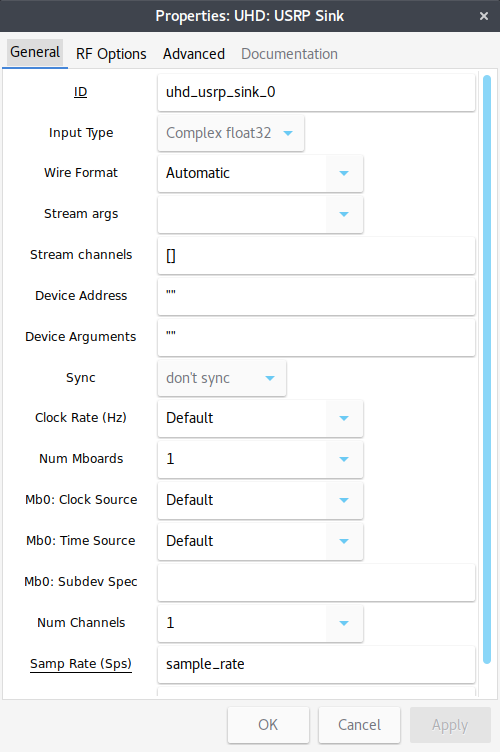
\includegraphics[width=0.4\textwidth]{figures/usrp_sink_general.png}
				\label{fig:usrp_sink_general}}
			\subfigure[USRP\_Sink设置:RF Options]{%
				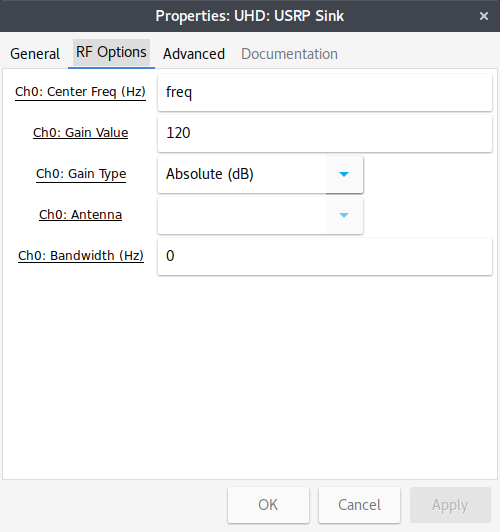
\includegraphics[width=0.4\textwidth]{figures/usrp_sink_rf_options.png}
				\label{fig:usrp_sink_rf_options}} \\
		\end{figure}
		\par USRP\_Sink模块的通用设置如图\ref{fig:usrp_sink_general}
		\par 其中常用的是以下两个参数:
		\par $\bullet$ Device Address
		\par 用来指定设备地址,可以通过执行\lstinline[language=sh]{uhd_find_devices}来查看已连接的设备地址,如果留空将默认使用第一个设备。
		\par $\bullet$ Samp Rate(Sps)
		\par 采样率,指每秒发送至USRP的数据量,同时也决定了发送信号的带宽,在I5-3337U的设备上可以取得的最大采样率为5MHz,过高的采样率会导致电脑无法处理而无法发送信号。
		\par USRP\_Sink模块的RF设置如图\ref{fig:usrp_sink_rf_options}
		\par 其中常用的为以下参数:
		\par $\bullet$ Center Freq(Hz)
		\par 中心频率,即发射频率。
		\par $\bullet$ Gain Value
		\par 增益,最高约可以调制120dB,通常使用70$\sim$90dB即可。
		\par $\bullet$ Antenma
		\par 天线,可以选择USRP发射或者接收的天线。
